%* 
%* ------------------------------------------------------------------
%* Model Railroad System by Deepwoods Software
%* ------------------------------------------------------------------
%* PrintingATimetable.tex - Printing a timetable
%* Created by Robert Heller on Tue Mar  5 08:40:57 2002
%* ------------------------------------------------------------------
%* Modification History: $Log$
%* Modification History: Revision 1.2  2004/04/14 23:22:17  heller
%* Modification History: Updated documentation.
%* Modification History:
%* Modification History: Revision 1.1  2002/11/09 21:21:07  heller
%* Modification History: Time Table User Manual
%* Modification History:
%* ------------------------------------------------------------------
%* Contents:
%* ------------------------------------------------------------------
%*  
%*     Model RR System, Version 2
%*     Copyright (C) 1994-2002  Robert Heller D/B/A Deepwoods Software
%* 			51 Locke Hill Road
%* 			Wendell, MA 01379-9728
%* 
%*     This program is free software; you can redistribute it and/or modify
%*     it under the terms of the GNU General Public License as published by
%*     the Free Software Foundation; either version 2 of the License, or
%*     (at your option) any later version.
%* 
%*     This program is distributed in the hope that it will be useful,
%*     but WITHOUT ANY WARRANTY; without even the implied warranty of
%*     MERCHANTABILITY or FITNESS FOR A PARTICULAR PURPOSE.  See the
%*     GNU General Public License for more details.
%* 
%*     You should have received a copy of the GNU General Public License
%*     along with this program; if not, write to the Free Software
%*     Foundation, Inc., 675 Mass Ave, Cambridge, MA 02139, USA.
%* 
%*  
%* 

\chapter{Printing A Timetable}
\label{chapt:PrintingATimetable}

The {\tt Make Time Table} button and the {\tt Print\ldots\ } menu item
on the {\tt File} menu on the main GUI (see
Chapter~\ref{chapt:MainGUI}), creates a hard copy time table from your
chart.  This time table will list all of your trains, with arrival and
departure times at each station.

Actually, a hard copy is not directly created.  Instead, a \LaTeX\ file
is created.  Under UNIX and MS-Windows, \LaTeX\ can be run as a
subprocess, or you can manually run \LaTeX\ later.  You might even want
to edit the generated \LaTeX\ file, if you wish to add extra
information or fine tune the formatting.

\section{The first step: Time Table generation parameters}

\begin{figure}[h] 
\begin{centering} 
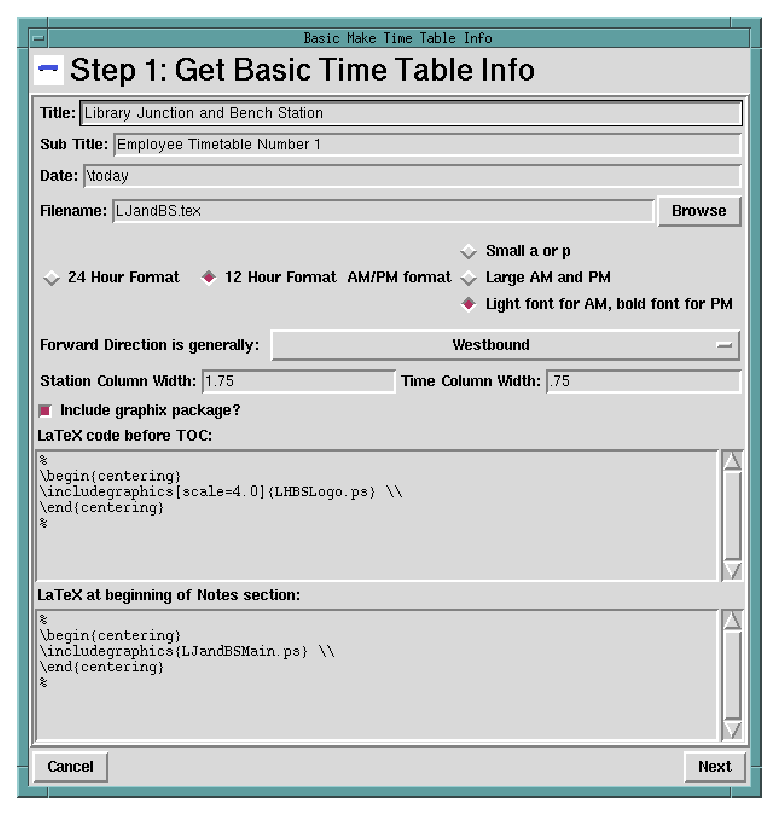
\epsfig{file=TimeTable/getBasicTimeTableInfo.ps}\\
\caption{Step 1: Get Basic Time Table Info dialog box.} 
\label{fig:getBasicTimeTableInfo}
\end{centering} 
\end{figure} When the {\tt Make Time Table} button\footnote{Or the {\tt Print\ldots\
} menu item on the {\tt File} menu.} is clicked on, you will first be
asked if you wish to load a set of previously saved Time Table
generation parameters.  After optionally loading these saved
parameters, the first (basic) set of time table generation parameters
are collected with the ``Step 1: Get Basic Time Table Info'' dialog
box, shown in Figure~\ref{fig:getBasicTimeTableInfo}.  This dialog box
collects the title, subtitle, date, filename, time format, general
layout direction and some column with information\footnote{In inches}. 
Also you can select the inclusion of the graphix \LaTeX\  package,
which allows for including graphical elements.  Also collected are
\LaTeX\ fragments to place before the Table Of Contents (such as your
railroad's logo) and to place at the beginning of the Notes section
(such as a route map).


If your time table won't fit on a single page, and unless you only run a
few trains per session, it won't, a second dialog box is pop-up after you
click {\tt Next} on the first dialog box.  The is the ``Step 2: Get
Multiple Table Time Table Info'' dialog box, shown in
Figure~\ref{fig:multipleTimeTableInfo}.  This dialog box gets
information relating to multiple pages of output, including whether to
generate single or double sided formatted output, whether to generate a
table of contents and how to group trains.

\begin{figure}
\begin{centering}
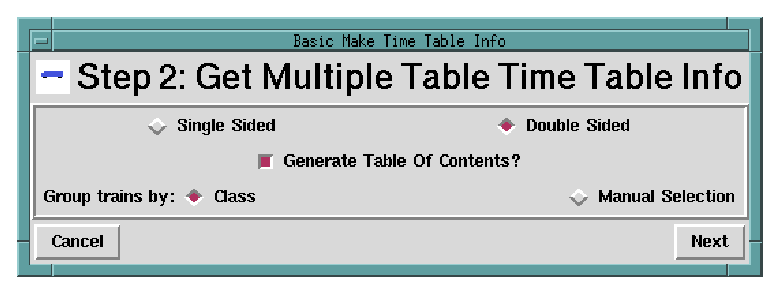
\epsfig{file=TimeTable/multipleTimeTableInfo.ps}\\
\caption{Step 2: Get Multiple Table Time Table Info dialog box.}
\label{fig:multipleTimeTableInfo}
\end{centering}
\end{figure}

\section{The second step: Grouping trains}

When printing a large set of schedules, you will be printing multiple
time tables, each for some grouping of trains.  There are two grouping
options, grouping by class and grouping manually.  Grouping by class is
easier, but only works properly if you don't have too many trains in a
given class.  Otherwise you will need to group manually.

\subsection{Grouping by class}

\begin{figure}[h]
\begin{centering}
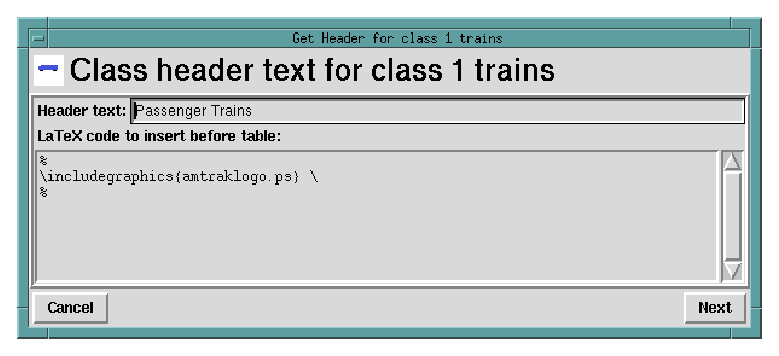
\epsfig{file=TimeTable/classGroupHeader.ps}\\
\caption{Class header text dialog box.}
\label{fig:classGroupHeader}
\end{centering}
\end{figure} When you select to group by class, a small dialog box,
like the one shown in Figure~\ref{fig:classGroupHeader}, is pop-up up
when each class is processed.  This dialog box allows you to specify a
header and some \LaTeX\ code to go at the top of the time table for the
time table for the specified class of trains.



\subsection{Grouping Manually}

When you select to group manually, the dialog box shown in
Figure~\ref{fig:manualGroup}.  This dialog box contains two lists: the
trains yet to be including in a time table and a list of trains in a
time table group.  You select one or more trains in one list and move
them to the other list using either of the \verb"<=" or \verb"=>"
buttons.  Once you have an acceptable group, you fill in the group
heading and select the {\tt Make Table} button.  Typically, a group
might be a related set of trains, such as the morning commuter trains.

\begin{figure}
\begin{centering}
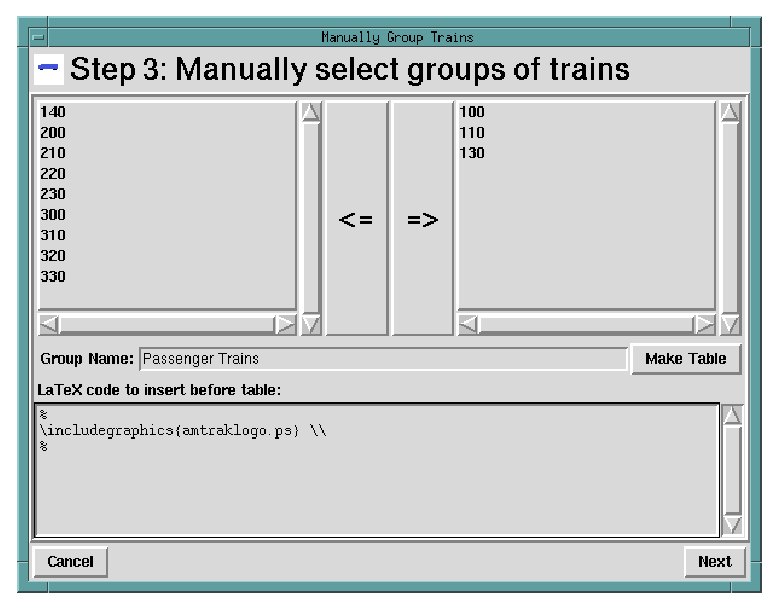
\epsfig{file=TimeTable/manualGroup.ps}\\
\caption{Manually Group Trains dialog box.}
\label{fig:manualGroup}
\end{centering}
\end{figure}   

\section{Running \LaTeX}

After the \LaTeX\ file has been generated, you will be asked if you want
to run \LaTeX.\footnote{Except under MacOS 9 or earlier.}  A series of
subprocess pop-up windows showing the progress of the subprocess runs of
\LaTeX\ and optionally dvidvi and dvips will be displayed.  You can also
skip this part and run \LaTeX\ and so on at a later time.



